% =========================
% APPENDIX
% =========================
\appendix


% ============================================================
% APPENDIX: Observation Terms
% % ============================================================
\subsection{Observation Terms}
\label{app:obs_terms}

\subsubsection{Notation and frames}
All relative geometric quantities are expressed in the robot base frame unless stated otherwise.
For WB, $p_r$ denotes the robot base position and $p_b$ the pushable object position.
For AM, $p_{ee}$ denotes the end-effector (fingertip) position, and $R_{bo}$ denotes the pushable rotation in the base frame.
We use $d_{rb}=\|p_r-p_b\|$ and $d_{bg}=\|p_b-p_g\|$ for robot--object and object--goal distance, respectively.
Yaw error is $e_\psi=\wrap(\psi_g-\psi_b)$.

% =================================
% WB observation table (grouped)
% ================================
\begin{table}[h]
\centering
\caption{\textbf{WB policy observations (high-level).}}
\label{tab:obs_wb}
\footnotesize
\setlength{\tabcolsep}{3pt}
\renewcommand{\arraystretch}{1.08}
\begin{tabular}{l c}
\toprule
\textbf{Observation term} & \textbf{Dim.}\\
\midrule
% \multicolumn{2}{l}{
% \textit{Robot base state}}\\
Base linear velocity ($v_{\text{base}}$) & 3\\
Base angular velocity ($\omega_{\text{base}}$) & 1\\
Projected gravity ($g_{\text{base}}$) & 3\\
Previous action ($a_{t-1}$) & 3\\
\addlinespace[0.25em]\hline\addlinespace[0.15em]
% \multicolumn{2}{l}{\textit{Task geometry (planar)}}\\
Robot--object relative vector (xy) & 2\\
Object--goal relative vector in base frame (xy) & 2\\
Object--goal distance ($d_{bg}$) & 1\\
Pushable heading in base frame & 2\\
Goal heading in base frame & 2\\
\addlinespace[0.25em]\hline\addlinespace[0.15em]
% \multicolumn{2}{l}{\textit{Object motion (planar)}}\\
Object planar velocity in base frame (xy) & 2\\
Speed toward goal ($v_{\parallel g}$) & 1\\
Tangential speed ($v_{\perp g}$) & 1\\
\addlinespace[0.25em]\hline\addlinespace[0.15em]
\textit{Low-level prior (frozen): locomotion-policy obs} & 48\\
\bottomrule
\end{tabular}
\end{table}

% ==========================
% AM observation table (grouped)
% ============================
\begin{table}[t]
\centering
\caption{\textbf{AM policy observations (high-level).}}
\label{tab:obs_am}
\scriptsize
\setlength{\tabcolsep}{3pt}
\renewcommand{\arraystretch}{1.08}
\begin{tabular}{l c}
\toprule
\textbf{Observation term} & \textbf{Dim.}\\
\midrule
% \multicolumn{2}{l}{
% % \textit{Robot base + arm state}
% }\\
Base linear velocity ($v_{\text{base}}$) & 3\\
Base angular velocity ($\omega_{\text{base}}$) & 3\\
Projected gravity ($g_{\text{base}}$) & 3\\
Arm joint positions (relative) & 6\\
Arm joint velocities & 6\\
Previous action ($a_{t-1}$) & 9\\
\addlinespace[0.25em]\hline\addlinespace[0.15em]
% \multicolumn{2}{l}{
% % \textit{Task geometry (3D)}
% }
End-effector to object vector in base frame & 3\\
Object to goal vector in base frame & 3\\
Object rotation matrix in base frame ($R_{bo}$) & 9\\
Goal rotation in object frame ($R_{og}$) & 9\\
\addlinespace[0.25em]\hline\addlinespace[0.15em]
Privileged encoder & 16\\
\bottomrule
\end{tabular}
% \vspace{-0.8em}
\end{table}

\subsubsection{Remarks.}
WB uses compact planar features (robot--object--goal geometry and object planar motion) together with base state.
AM augments these with end-effector geometry and arm proprioception for contact placement and fine steering.
Privileged object features are logged for analysis and can optionally supervise object-conditioned encoders.

% =================================
% APPENDIX: Reward Terms
% ==============================

\subsection{Reward Terms}
\label{sec:reward_terms}

\subsubsection{Whole-body pushing reward structure}
We group the WB reward into (i) a \emph{core objective} consisting of an intrinsic term $r_{\mathrm{int}}$ and an extrinsic term adapted from \cite{Jeon2023WholeBodyQuadruped},
and (ii) additional shaping/regularization terms (Table~\ref{tab:wb_reward_summary}).
The intrinsic term is composed of base components $r_1\ldots r_6$ with coefficients (Table~\ref{tab:wb_jeon_components}).

% ---------------- WB reward summary ----------------
\begin{table}[t]
\centering
\caption{\textbf{Whole-body pushing (WB): reward summary.}}
\label{tab:wb_reward_summary}
\scriptsize
\setlength{\tabcolsep}{3pt}
\renewcommand{\arraystretch}{1.18}
\begin{tabular}{p{2.55cm} p{4.65cm} c}
\toprule
\textbf{Term} & \textbf{Definition} & \textbf{$w$} \\
\midrule
\multicolumn{3}{l}{\textit{Core objective (task completion)}}\\
Intrinsic  & $r_{int}(t)$ (see Table.~\ref{tab:wb_jeon_components}) & 0.15 \\
Extrinsic  & $\log\!\big(\norm{G_g-G_b}_2 + 0.05\big)$ & 6 \\
\addlinespace[0.25em]\hline\addlinespace[0.15em]
\multicolumn{3}{l}{\textit{Approach and progress shaping}}\\
Behind-box &
$r_{\mathrm{b}}=\big(\max(0,-\hat u_{rb}^{\top}\hat u_{bg})\big)^2\,\mathbf{1}[d_{rb}<d_e]$
& 1.0 \\
Toward-goal vel. &
$r_{v}=\clip(v_b^{\top}\hat u_{bg},0,1)\,\mathbf{1}[d_{rb}<d_e]$
& 2.0 \\
Progress &
$r_{\Delta d}=\clip(d_{bg}^{t-1}-d_{bg}^{t},-\delta,\delta)\,\mathbf{1}[d_{rb}<d_e]$
& 8.0 \\
\addlinespace[0.25em]\hline\addlinespace[0.15em]
\multicolumn{3}{l}{\textit{Near-goal precision}}\\
Pose precision &
$r_{xy}=\exp\!\big(-d_{bg}^2/\sigma_{xy}^2\big)\,\mathbf{1}[d_{bg}<d_{xy}]$
& 3.0 \\
Yaw precision &
$r_{\psi}=\exp\!\big(-e_{\psi}^2/\sigma_{\psi}^2\big)\,\mathbf{1}[d_{bg}<d_{\psi}]$
& 2.5 \\
Settle &
$r_{\mathrm{settle}}=\exp(-\|v_b\|/\sigma_v)\,\mathbf{1}[d_{bg}<d_s]$
& 2.0 \\
Tangent penalty &
$r_{\mathrm{tan}}=-\|v_b-(v_b^{\top}\hat r)\hat r\|^2\,\mathbf{1}[d_{bg}<d_t]$
& 1.0 \\
Success dwell &
$r_{\mathrm{dwell}}=\mathbf{1}[c_t\ge K]$ (Eq.~\ref{eq:wb_dwell})
& 20.0 \\
Micro precision &
$r_{\mathrm{micro}}=\exp\!\big(-d_{bg}^2/\sigma_m^2\big)\,\mathbf{1}[d_{bg}<d_m]$
& 12.0 \\
\addlinespace[0.25em]\hline\addlinespace[0.15em]
\multicolumn{3}{l}{\textit{Stability and motion regularization}}\\
Upright dense &
$r_{\mathrm{up}}=\clip(\cos\theta_{\mathrm{up}},0,1)$
& 0.05 \\
Upright threshold &
$r_{\mathrm{up\text{-}pen}}=-\ReLU(\tau-\cos\theta_{\mathrm{up}})$
& 2.0 \\
\bottomrule
\end{tabular}
\vspace{-0.6em}
\end{table}





% ---------------- WB Jeon-style components + intrinsic (combined) ----------------
\begin{table}[t]
\centering
\caption{\textbf{WB: intrinsic components.}}
\label{tab:wb_jeon_components}
\scriptsize
\begin{tabular}{@{}p{0.95cm} p{4.75cm} c@{}}
\toprule
\textbf{Term} & \textbf{Definition} & \textbf{Coeff.} \\
\midrule
$r_1$ & $\exp\!\big(-\norm{p_r-p_b}_2\big)$ & 1 \\
$r_2$ & $\log\!\big(\norm{G_g-G_b}_2 + 0.05\big)$ & 4 \\
$r_3$ & $\exp\!\big(-\phi_{r,x}^{\top} v_b\big)$ & 1 \\
$r_4$ & $\exp\!\big(-(p_g-p_b)^{\top} v_b\big)$ & 1 \\
$r_5$ & $\exp\!\big(-\norm{a_t-a_{t-1}}_2\big)$ & 2 \\
$r_6$ & $\exp\!\big(-\norm{a_t-2a_{t-1}+a_{t-2}}_2\big)$ & 3 \\
\midrule
$r_{\mathrm{int}}(t)$ &
$\displaystyle
\begin{cases}
r_{Ji}(t-1), & d_{bg}<0.2,\\
k_7\,(r_1+r_3+r_4+r_5+r_6), & \text{otherwise},
\end{cases}$
& -- \\
\bottomrule
\end{tabular}
\end{table}




% \noindent\textit{Success dwell counter.}
% \begin{IEEEeqnarray}{rCl}
% c_t &=&
% \begin{cases}
% c_{t-1}+1, & d_{bg}<\epsilon_p \wedge |e_\psi|<\epsilon_\psi,\\
% 0, & \text{otherwise}.
% \end{cases}\IEEEyesnumber\label{eq:wb_dwell}
% \end{IEEEeqnarray}



\textit{WB notation}
$d_{rb}=\norm{p_r-p_b}$, $d_{bg}=\norm{p_b-p_g}$,
$\hat u_{rb}=\frac{p_r-p_b}{\norm{p_r-p_b}}$, $\hat u_{bg}=\frac{p_g-p_b}{\norm{p_g-p_b}}$,
$e_\psi=\wrap(\psi_g-\psi_b)$.
$\phi_{r,x}$ is the robot-forward unit vector in the object frame (as in the original formulation).
Dwell uses $(\epsilon_p,\epsilon_\psi,K)$.
% \normalsize

% ---------------- AM reward terms (style-matched) ----------------
\subsubsection{Arm-mediated pushing reward structure.}
\begin{table}[t]
\centering
\caption{\textbf{Arm-mediated pushing (AM): reward terms.}}
\label{tab:am_reward_terms}
\scriptsize
\setlength{\tabcolsep}{3pt}
\renewcommand{\arraystretch}{1.10}
\begin{tabular}{@{}p{2.0cm}p{\dimexpr\columnwidth-2.0cm-0.55cm-4\tabcolsep\relax}p{0.55cm}@{}}
\toprule
\textbf{Term} & \textbf{Definition} & \textbf{$w$}\\
\midrule
\multicolumn{3}{@{}l}{\textit{Goal pose + progress}}\\
Pose match &
$r_{\text{pose}}=\exp\!\big(-e_{\text{kp}}^{2}/\sigma_3^{2}\big)$
& 3.0\\
Reach shaping &
$r_{\text{reach}}=\exp\!\big(-\|p_{ee}-p_{\text{tgt}}\|^{2}/\sigma_1^{2}\big)$
& 2.5\\
Velocity to goal &
$r_{\text{vel}}=\exp\!\big(-(1-\alpha)^{2}/\sigma_2^{2}\big)$
& 0.156\\
\addlinespace[0.20em]\midrule\addlinespace[0.10em]
\multicolumn{3}{@{}l}{\textit{Stability + safety}}\\
Object stability &
$r_{\text{stab}}=\sigmoid\!\big(s(\cos\theta-\cos\theta_{\lim})\big)$
& 0.4\\
Undesired contacts &
$r_{\text{col}}=-\sum_{b\in\mathcal{B}_{\neg ee}}\mathbf{1}\!\left[\|F_b\|>\tau\right]$
& -0.05\\
\bottomrule
\end{tabular}
\end{table}


\paragraph{AM implementation details (symbols).}
$e_{\text{kp}}=\frac{1}{K}\sum_{k=1}^{K}\|q_k^{w}-g_k^{w}\|$ (keypoint error);
$\alpha=\clip(\hat v_{xy}^{\top}\hat u_{og},0,1)$ (planar velocity-to-goal alignment);
$\cos\theta=\hat z_o^\top\hat z_w$ with $\cos\theta_{\lim}=\cos(20^\circ)$.
Reach uses $p_{ee}$ and sampled surface target $p_{\text{tgt}}$.
Safety checks contact forces on disallowed bodies $\mathcal{B}_{\neg ee}$.
We use $\sigma_1{=}0.5916,\ \sigma_2{=}0.7071,\ \sigma_3{=}0.7746,\ \tau{=}0.2$.





% ============================================================
% APPENDIX: Low-level locomotion prior
% ============================================================
\subsection{Low-level locomotion prior.}
End-to-end loco-manipulation is difficult because a single policy must learn both (i) dynamic balance/gait control and
(ii) task-driven contact interactions. This coupling can destabilize training: exploration for pushing often induces falls,
while stabilization behaviors can dominate the learning signal. We therefore use a pretrained low-level locomotion prior
to provide stable gait and body regulation, and learn task-level decision making on top.

Following ~\cite{Draxler2025ReLIC}, we pretrain a Spot locomotion policy in simulation while the arm
tracks randomly sampled 3D end-effector targets (Fig.~\ref{fig:lowlevel_relic_training}). Targets are resampled online to
generate diverse arm motions; an IK/PD controller tracks them within joint limits, inducing disturbances that the base
policy learns to reject. After pretraining, the locomotion policy is \emph{frozen} and used as the stabilizing layer in all
pushing experiments. 

% We do not use a three-leg manipulation mode: manipulation is performed only through the arm/end-effector, and the legs are used solely for locomotion and balance.
\begin{figure}[h]
    \centering
    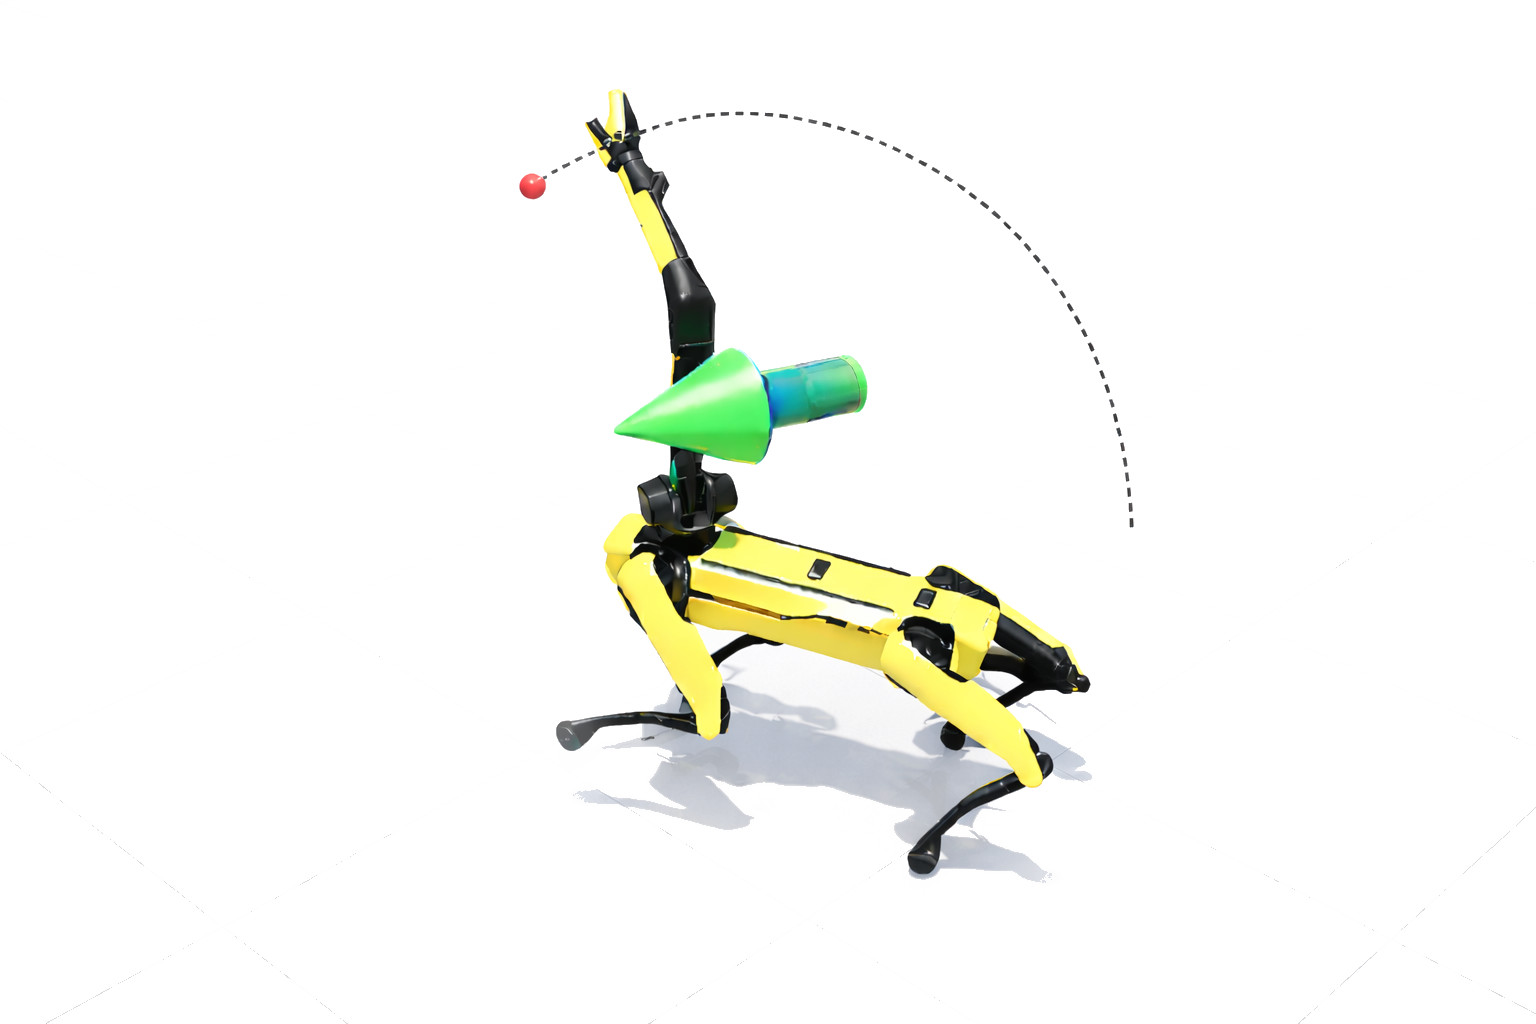
\includegraphics[width=0.9\linewidth]{Images/relic.jpg}
    \caption{\textbf{Low-level locomotion prior pretraining.}
    Spot is trained to locomote while the arm tracks randomly resampled 3D end-effector targets (red), producing diverse arm motions and disturbances; the resulting locomotion policy is then frozen and used as a stabilizing prior for pushing.}
    \label{fig:lowlevel_relic_training}
\end{figure}